\documentclass{scrartcl}
\usepackage[usenames,dvipsnames,svgnames]{xcolor}
\usepackage[shortlabels]{enumitem}
\usepackage[framemethod=TikZ]{mdframed}
\usepackage{amsmath,amssymb,amsthm}
\usepackage{epigraph}
\usepackage[colorlinks]{hyperref}
\usepackage{microtype}
\usepackage{mathtools}
\usepackage[headsepline]{scrlayer-scrpage}
\usepackage{thmtools}
\renewcommand{\epigraphsize}{\scriptsize}
\renewcommand{\epigraphwidth}{60ex}
\addtolength{\textheight}{3.14cm}
\ihead{\footnotesize\textbf{Geometry Review}}
\ohead{\footnotesize \today}
\providecommand{\clubs}[1]{$#1\clubsuit$}
\providecommand{\ol}{\overline}
\providecommand{\eps}{\varepsilon}
\providecommand{\half}{\frac{1}{2}}
\providecommand{\dang}{\measuredangle} %% Directed angle
\providecommand{\CC}{\mathbb C}
\providecommand{\FF}{\mathbb F}
\providecommand{\NN}{\mathbb N}
\providecommand{\QQ}{\mathbb Q}
\providecommand{\RR}{\mathbb R}
\providecommand{\ZZ}{\mathbb Z}
\providecommand{\dg}{^\circ}
\providecommand{\ii}{\item}
\providecommand{\alert}[1]{{\sffamily\textbf{\textcolor{blue}{#1}}}}

\reversemarginpar


\mdfdefinestyle{mdbluebox}{roundcorner=10pt,innerbottommargin=9pt,
	linecolor=blue,backgroundcolor=TealBlue!5,}
\declaretheoremstyle[headfont=\sffamily\bfseries\color{MidnightBlue},
mdframed={style=mdbluebox},]{thmbluebox}

\mdfdefinestyle{mdredbox}{frametitlefont=\bfseries,innerbottommargin=8pt,
	nobreak=true,backgroundcolor=Salmon!5,linecolor=RawSienna,}
\declaretheoremstyle[headfont=\bfseries\color{RawSienna},
mdframed={style=mdredbox},headpunct={\\[3pt]},postheadspace=0pt,]{thmredbox}

\mdfdefinestyle{mdgreenbox}{linecolor=ForestGreen,backgroundcolor=ForestGreen!5,
	linewidth=2pt,rightline=false,leftline=true,topline=false,bottomline=false,}
\declaretheoremstyle[headfont=\bfseries\sffamily\color{ForestGreen!70!black},
mdframed={style=mdgreenbox},headpunct={ --- },]{thmgreenbox}

\mdfdefinestyle{mdorangebox}{linecolor=RedOrange,backgroundcolor=RedOrange!5,
	linewidth=2pt,rightline=false,leftline=true,topline=false,bottomline=false,}
\declaretheoremstyle[headfont=\bfseries\sffamily\color{RedOrange!70!black},
mdframed={style=mdorangebox},headpunct={ --- },]{thmorangebox}

\mdfdefinestyle{mdblackbox}{linecolor=black,backgroundcolor=RedViolet!5!gray!5,
	linewidth=3pt,rightline=false,leftline=true,topline=false,bottomline=false,}
\declaretheoremstyle[mdframed={style=mdblackbox}]{thmblackbox}

\declaretheorem[style=thmredbox,name=Problem,numberwithin=subsection]{problem}
\declaretheorem[style=thmredbox,name=Example,numberwithin=subsection]{example}
\declaretheorem[style=thmredbox,name=$\bigstar$ Problem,sibling=problem]{niceprob}

\declaretheorem[style=thmbluebox,name=Theorem,sibling=example]{theorem}
\declaretheorem[style=thmbluebox,name=Proposition,sibling=example]{prop}
\declaretheorem[style=thmbluebox,name=Corollary,sibling=theorem]{corollary}
\declaretheorem[style=thmbluebox,name=Lemma,sibling=theorem]{lemma}
\declaretheorem[style=thmbluebox,name=Theorem,numbered=no]{theorem*}
\declaretheorem[style=thmbluebox,name=Lemma,numbered=no]{lemma*}

\declaretheorem[style=thmgreenbox,name=Claim,numberwithin=theorem]{claim}
\declaretheorem[style=thmgreenbox,name=Claim,numbered=no]{claim*}
\declaretheorem[style=thmgreenbox,name=Definition,sibling=theorem]{definition}
\declaretheorem[style=thmgreenbox,name=Definition,numbered=no]{definition*}

\declaretheorem[style=thmblackbox,name=Remark,sibling=theorem]{remark}
\declaretheorem[style=thmblackbox,name=Remark,numbered=no]{remark*}

\declaretheorem[style=thmorangebox,name=Warning,sibling=theorem]{warning}
\declaretheorem[style=thmorangebox,name=Note,numbered=no]{note}
\declaretheorem[style=thmblackbox,name=Exercise,numbered=no]{exercise}

\usepackage{graphicx}
\usepackage{todonotes}

\newenvironment{soln}{\begin{proof}[Solution]}{\end{proof}}
\newenvironment{walkthrough}{\noindent\textbf{Walkthrough.}}{}
\newlist{walk}{enumerate}{3}
\setlist[walk]{label=\bfseries (\alph*)}
\usepackage{todonotes}

\providecommand{\pow}{\operatorname{Pow}}
\providecommand{\vocab}[1]{{\textbf{\textcolor{ForestGreen}{#1}}}}

\title{GeoGebra 101}
\author{Aditya Pahuja}
\date{\today}
\begin{document}
\maketitle

Have you been doing way too much geometry?
Are you spending hours painstakingly drawing circles with a compass?
Are you afraid of this newfangled technology that kids these days use???

Well, fear no more: here's a short guide on using GeoGebra
to efficiently create geometry diagrams.

\tableofcontents
\pagebreak

\section{Version}
This guide uses GeoGebra Classic 5,
which can be installed \href{https://www.geogebra.org/download}{here}.
Most things should probably work in other versions too, I guess?

\section{What is GeoGebra?}
GeoGebra is a dynamic geometry software:
you can define objects based on other objects,
such as a line through two points,
and then moving around the defining points of the line
also moves the line! (Doing this in, say, Desmos would be painful.)
This robustness makes GeoGebra a handy tool for plane geometry,
since it allows you to effortlessly perturb a diagram and verify conjectures.
There are also graphing capabilities (similar to Desmos) and 3D geometry tools,
but those are not of interest here.

\section{Starting Points}
Before we start making pictures, look at the GeoGebra interface.
There are some pre-built tools, settings at the top,
a small Graphics tab, and an Algebra tab on the left.
These comprise the main items you'll be interacting with.

Now, I could go through each and every command that you'd normally use,
but that's both tedious and redundant due to the appendix.
In lieu of this, awa.

\section{Tweaking Visual Settings}
In the Graphics tab, assuming you have the Move tool selected,
you should see the following list of options:
\begin{figure}[h]
	\centering
	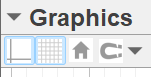
\includegraphics[width=0.2\linewidth]{toggleGridAxes}
	\label{fig:togglegridaxes}
\end{figure}

The two options on the left allow you to toggle the grid and the axes;
the home icon repositions your view and the magnet icon
lets you choose if placed objects snap to points on the grid.

If you want to mess with more settings relating to the grid or axes,
click this gear icon in the top right and then click Graphics:
\begin{figure}[h]
	\centering
	
\includegraphics[width=0.2\linewidth]{moreSettings}
	\label{fig:moresettings}
\end{figure}

\section{Appendix: A complete list of useful commands}
Let me know if I missed a frequently-used command!

\begin{itemize}
	\ii awa
	\ii awa
	\ii awa
\end{itemize}

\end{document}